\documentclass[handout, aspectratio=169]{beamer}

%Packages
\usepackage[utf8]{inputenc}
\usepackage{pgfpages}
\usepackage{graphicx}
\usepackage[italian]{babel}
\usepackage{amsmath}

\title[CRYPTO1]{CRYPTO1 Stream cypher}
\author[Stefano Fontana]{Stefano Fontana, Mat.727199}
\institute[]{Università degli studi di brescia}
\date{A.A. 2021/2022}

%Settings
\usetheme{metropolis}
\useoutertheme[hideothersubsections,left]{sidebar}
\setbeamercovered{transparent}
\setbeamertemplate{navigation symbols}{}

\bibliographystyle{alpha}

\graphicspath{{figures/}}

\makeatletter
    \setbeamertemplate{sidebar left}
    {
        \beamer@tempdim=\beamer@sidebarwidth%
        \advance\beamer@tempdim by -6pt%
        \insertverticalnavigation{\beamer@sidebarwidth}%
        \vfill
        \ifx\beamer@sidebarside\beamer@lefttext%
        \else%
            \usebeamercolor{normal text}%
            \llap{\usebeamertemplate***{navigation symbols}\hskip0.1cm}%
            \vskip1pt%
        \fi%
    }%

    \ifx\beamer@sidebarside\beamer@lefttext%
        {%
            \vfill%
            \llap{\usebeamertemplate***{navigation symbols}\hskip0.1cm}%
            \vskip1pt
        }
    \fi

    \setbeamertemplate{section in sidebar}%{sidebar theme}
    {%
    \vbox{%
        \beamer@sidebarformat{3pt}{section in sidebar}{\insertsectionheadnumber~\insertsectionhead}%
    }%
    }
    \setbeamertemplate{section in sidebar shaded}%{sidebar theme}
    {%
    \vbox{%
        \vskip1ex%
        \beamer@sidebarformat{3pt}{section in sidebar shaded}{\insertsectionheadnumber~\insertsectionhead}%
    }%
    }
\makeatother
\usepackage{pgfpages}
\hypersetup{hidelinks}

\pgfpagesuselayout{2 on 1}[a4paper, border shrink=8mm]

\setbeameroption{show notes on second screen=bottom}

\newlength{\parskipbackup}
\setlength{\parskipbackup}{\parskip}
\newlength{\parindentbackup}
\setlength{\parindentbackup}{\parindent}
\newcommand{\baselinestretchbackup}{\baselinestretch}

\usetemplatenote{\rmfamily%
  \setlength{\parindent}{1em} \setlength{\parskip}{1ex}%
  \renewcommand{\baselinestretch}{1}%
  \noindent \insertnote%

  \setlength{\parskip}{\parskipbackup}%
  \setlength{\parindent}{\parindentbackup}%
  \renewcommand{\baselinestretch}{\baselinestretchbackup}%
}

\pgfpageslogicalpageoptions{1}{border code=\pgfusepath{stroke}}

\AtBeginSection[]{
    \stepcounter{page}
}

\begin{document}
  \begin{frame}[plain]
    \maketitle
\end{frame}

\section{Sommario}
\begin{frame}[allowframebreaks]
    \frametitle{Sommario}
    \setbeamertemplate{section in toc}[sections numbered]
    \tableofcontents
\end{frame}
\note{
    %\begin{enumerate}
    %X    \item Tag NFC e ISO14443
    %    \begin{enumerate}
    %X        \item UUID \textit{Questo sarà necessario perchè l'uuid appare come parametro di inizializzazione dello stream cipher}
    %X        \item Struttura della memoria e processo di autenticazione per Mifare Classic
    %    \end{enumerate}
    %    \item Introduzione generale degli stream cipher
    %    \item Algoritmo CRYPTO1
    %    \begin{enumerate}
    %        \item Confronto con uno stream cypher ideale e vulnerabilità
    %        \item Vulnerabilità implementative
    %        \begin{enumerate}
    %X            \item valore del RNG del reader dipendente da numero di invocazioni
    %X            \item valore del RNG del tag dipendente solamente dal tempo di accensione
    %            \item LFSR state recovery
    %            \item LFSR rollback
    %        \end{enumerate}
    %        \item Vulnerabilità concettuali dell'algoritmo
    %        \begin{enumerate}
    %X            \item Nonce a 32bit effettivamente funzione di un valore a 16 bit
    %            \item La ``Filter function'' utilizza solo i bit dispari del LFSR
    %            \item Parity bit attacks
    %        \end{enumerate}
    %        \item Attacchi
    %        \begin{enumerate}
    %            \item Genuine reader attacks
    %            \item Genuine tag attack
    %            \item Eavesdropping
    %            \item https://github.com/DrSchottky/mfcuk
    %        \end{enumerate}
    %        \item Considerazioni per il miglioramento
    %        \begin{enumerate}
    %            \item Miglioramento del RNG
    %            \item Ridefinizione della ``Filter function''
    %            \item AES impl https://digital-library.theiet.org/content/journals/10.1049/ip-ifs\_20055006
    %            \item Considerazioni relative alla fattibilità e all'aumento del costo per tag
    %        \end{enumerate}
    %        \item Successori
    %        \begin{enumerate}
    %            \item Mifare Desfire
    %        \end{enumerate}
    %    \end{enumerate}
    %\end{enumerate}
}

\section{ISO14443}

\begin{frame}
    \frametitle{ISO14443a e NFC}
    \textbf{Cos'è NFC}\\
    Teconologia di comunicazione contactless (short range wireless)
    che permette dispositivi a basso costo\cite{coskun2013survey}

    \pause

    \textbf{Come funziona}
    \begin{itemize}
        \item<1-> Semplificando il tutto, la comunicazione NFC è equivalente a un trasformatore.
        \item<2-> la trasimissione dell'informazione avviene mediante ASK e Load Modulation\cite{instruments2014iso}
    \end{itemize}
\end{frame}
\note{
    La codifica dell'informazione avviene con una variante di  manchester encoding\cite{instruments2014iso}
    
    Uno dei principali vantaggi della tecnologia è che il tag può essere completamente passivo e alimentarsi grazie al campo magnetico generato dal tag, il quale causa induzione magnetica nella bobina del dispositivo.
}

\begin{frame}
    \begin{figure}
        \centering
        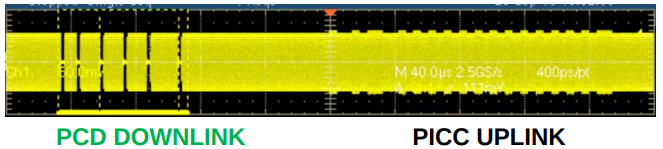
\includegraphics[width=0.85\textwidth]{ISO14443a_COM.png}
        \caption{Traccia della comunicazione tra dispositivo e lettore~\cite{instruments2014iso}}
        \label{fig:iso14443a-trace}
    \end{figure}
    Si noti come la frequenza della portante sia notevolmente elevata\pause

    Ciò permette di avere dei dispositivi (TAG) completyamente passivi alimentati dalla portante stessa.
\end{frame}
\note{
    Dall'immagine è possibile osservare come la trasmissione in downlink sia 100\% ASK, dove le tempistiche di bit
    sono notevolmente inferiori ai 13.56MHz della portante.
    Ciò permette al dispositivo di essere completamente passivo e di auto alimentarsi tramite l'effetto trasformatore
    causato dal coupling elettoromagnetico delle due induttanze.
    La trasmissione inversa, dal tag al lettore, di conseguenza non può avvenire allo stesso modo, essendo il tag non in grado di generare
    una portante.
    
    La soluzione è di variare l'impedenza collegata alla spira di ricezione nel tag in modo da utilizzare più corrente.
    Questo causerà una maggiore corrente nel lato trasmettitore che, mediante la resistenza interna di quest'ultimo, causerà una caduta
    di tensione leggibile e interpretabile.
}

\subsection{UUID e anticollisione}
\begin{frame}
    \frametitle{UUID e identificazione multipla di TAG}
    \begin{itemize}
        \item<1-> L'UUID è un codice di identificazione univoco che permette l'identificazione dei tag.
        Un generico tag ISO14443-compilant possiede un UUID di 10byte, ma varie implementazioni permettono di avere una lunghezza a partire da 4byte.\cite{nxpmifareuidhandling}
        \item<2-> Mediante il ciclo di identificazione e anticollisione è possibile ottenere la lista di tutti i tag presenti nelle vicinanze del lettore.
        \item<3-> Sarà poi possibile inviare comandi specifici a un solo tag mendiante il processo di selezione
    \end{itemize}
\end{frame}
\note{
    Secondo lo standard, durante il processo di discover (Denominato ``anticollision loop'') è possibile dostinguere i tag grazie ai loro id.

    È interessante notare, leggendo~\cite{nxpmifareev1datasheet}, che sono possibili più iterazioni del ciclo di anticollisione (CL1, CL2, CL3) dove ogni esecuzione incrementa il numero di byte che definiscono l'UUID.

    Risulta quindi che per una carta implementante tutti e tre i livelli di anticollisione l'UUID sarà \textbf{univoco} e lungo 80 bit; mentre per le carte con soli due livelli l'UUID sarà di 56 bit ma pur sempre \textbf{univoco}.
    L'unica implementazione dove il valore \textbf{non è garantito che sia univoco} è quella base da 32 bit.

    Il protocollo poi prosegue con un paradigma ``select and operate'',
    dove una sessione di comunicazione viene iniziata tramite l'UUID inviato dal lettore. A questo punto tutti i tag nella zona attiva rimarranno in stato IDLE ad eccezione del tag che è stato interpellato.
}

\subsection{Tag MIFARE Classic}
\subsubsection{Struttura della memoria}
\begin{frame}
    \frametitle{MIFARE Classic: Struttura della memoria}
    I tag MIFARE Classic sono tra i più \textbf{semplici} e \textbf{economici}:
    
    Il tag consiste in un piccolo frontend radio e logico che possa gestire la comunicazione
    e in una memoria non volatile dove salvare le configurazioni.\cite{nxpmifareev1datasheet}

    \begin{figure}
        \centering
        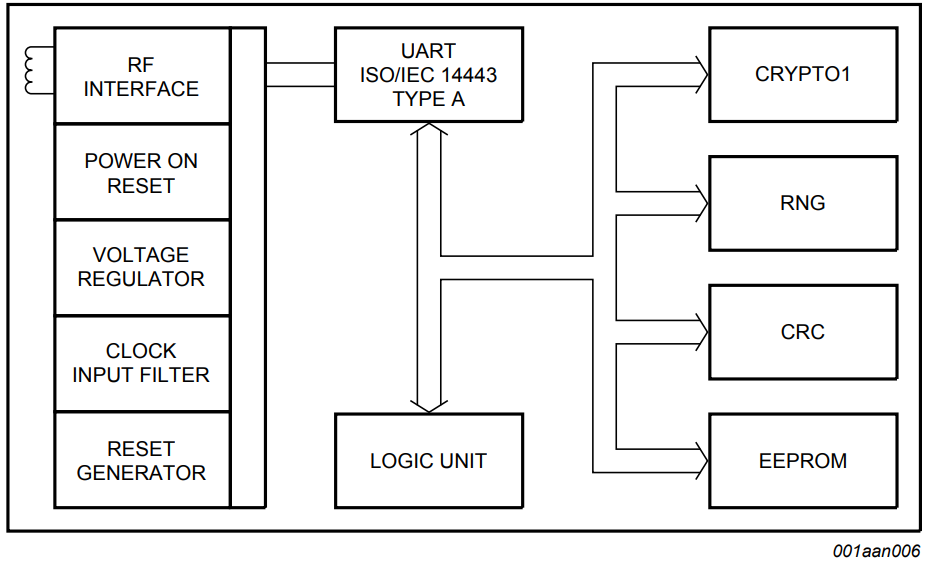
\includegraphics[width=0.3\textwidth]{MIFARE-EV1-INTERNAL_STRUCTURE.png}\cite{nxpmifareev1datasheet}
        \caption{Diagramma dei componenti interni a un chip MIFARE Classic}
        \label{fig:internal-mifare-block-diagram}
    \end{figure}
\end{frame}
\note{
    \footnotesize
    \begin{columns}
        \begin{column}{0.5\textwidth}
            La struttura di un tag MIFARE CLASSIC è da ritenersi interessante.
    
            Data il ridotto costo del dispositivo ne consegue una bassa complessità elettronica.
            Infatti esso è composto per una buona parte di componenti standard atti alla gestione della comunicazione e del chip in sè: L'interfaccia radio e il regolatore di tensione infatti sono gli unici componenti analogici presenti sul silicio.

            Successivamente si ha l'unità logica che ha il compito di gestira la comunicazione e vigilare sulle operazioni, ma quest'ultima non ha grande compessità. L'algoritomo utilizzato è di fatto molto contenuto ed è equivalente a una macchina a stati.

            È interessante notare come la gestione della memoria, in seguito descritta, sia ottimizzata al fine di ridurre i costi.
        \end{column}
        \begin{column}{0.5\textwidth}
            \begin{figure}
                \centering
                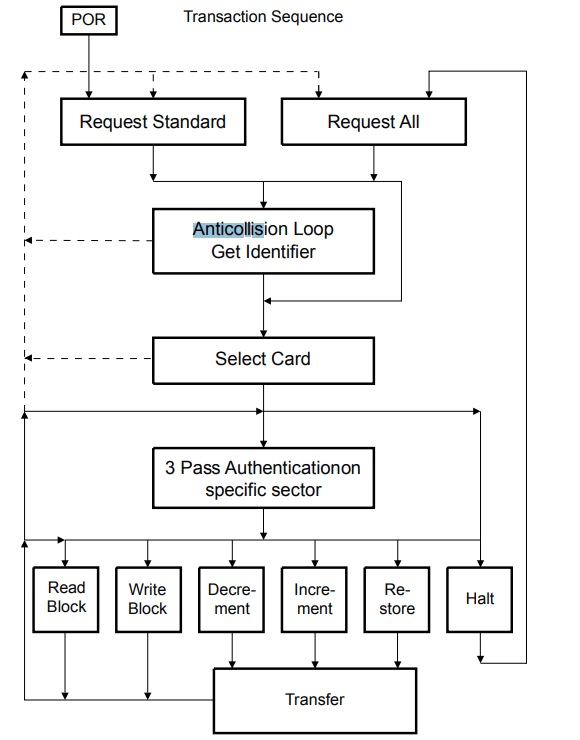
\includegraphics[width=.6\textwidth]{algo_mifare.png}
                \caption{Schema a blocchi della gestione logica di una transazione}
            \end{figure}
        \end{column}
    \end{columns}
}

\begin{frame}
    La memoria è divisa in \textbf{settori} e \textbf{blocchi}:
    \begin{itemize}
        \item <1-> 16 settori \texttt{[0-15]}
        \item <2-> 4 blocchi per settore \texttt{[0-3]}
        \item <2-> Solo tre blocchi per settore possono includere dati \texttt{[0-2]}
        \item <3-> Il blocco \texttt{0:0} è leggibile senza autenticazione, protetto in scrittura e contiene l'uuid e dati del produttore
        \item <4-> I blocchi \texttt{x:3} contengono le chiavi di scrittura e lettura (\textit{KeyA} e \textit{KeyB}), oltre che gli indicatori di protezione (access bits)
    \end{itemize}
\end{frame}
\note{
    È molto interessante notare come, al fine di mantenere bassi i costi di fabbricazione, le memorie sono le responsabili per i costi (e lo spazio su silicio) più elevati.

    Di conseguenza all'interno dei tag la memoria stessa viene utilizzata per il salvataggio delle chiavi di accesso e delle condizioni.

    È inoltre interessante notare come esistano due diverse chiavi di cifratura per ogni settore: questo è fatto al fine di permettere l'utilizzo diversificato del tag a fronte di un segreto condiviso diverso. Molte volte la chiave A è utilizzata per permettere la sola lettura dei blocchi (escluso quello contenente la chiave B), mentre la chiave B è una chiave master in grado di riprogrammare il tag.

    Bisogna però citare \cite{Courtois2009TheDS}, dove l'autore sottolinea come l'implementazione dell'algoritmo sia una ``waste of silicon'' data la caratteristica dell'offuscamento, dove funzioni identità sono implementate in modi diversi sul die. Questo, moltiplicato per il numero di tag prodotti un vero e proprio spreco di materiale.
}

\subsubsection{Lettura e scrittura}
\begin{frame}
    \frametitle{MIFARE Classic: Lettura e scrittura}
    Prima di effettuare qualunque azione sulla memoria è necessario autenticarsi con la chiave adatta al settore in questione.\pause

    Il processo di autentiocazione è chiamato \textit{``Three pass authentication sequence''}\cite{nxpmifareev1datasheet}
    e sfrutta un cifrario a flusso
\end{frame}
\note{
    Durante questa procedura il cifrario viene inizializzato in uno stato comune al fine di permettere una trasmissione riservata.
    Lo stato condiviso sfrutta la presenza di nonce casuali per assicurare l'unicità della comunicazione in modo da impedire correlzioni e attacchi replica.
}

\subsubsection{Three pass authentication sequence}
\begin{frame}
    \frametitle{Three pass authentication sequence\cite{garcia2008dismantling}}
    {
        \small
        \begin{columns}[onlytextwidth,T]
            \column{\dimexpr\textwidth-40mm-2mm}
                \begin{itemize}
                    \item <1-> Il tag entra nel campo magnetico del lettore e si accende
                    \item <2-> Protocollo di anticollisione (\textit{Non descritto}) e invio dell'UUID
                    \item <3-> Il lettore effettua una richiesta di autenticazione al blocco richiesto
                    \item <4-> Il tag ritorna un nonce \(n_t\) e lo trasmette in chiaro
                    \item <5-> Il lettore quindi invia il proprio nonce \(n_r\) e la risposta alla challenge \(a_r\)
                            cifrandoli mediante xoring con lo stream proveniente dal cifrario a flusso \(ks_1\) e \(ks_2\)
                    \item <6-> L'autenticazione si conclude con il tag che risponderà alla challenge del reader con \(a_t\) cifrato tramite \(ks_3\)
                \end{itemize}
            \column{40mm}
                \begin{figure}
                    \centering
                    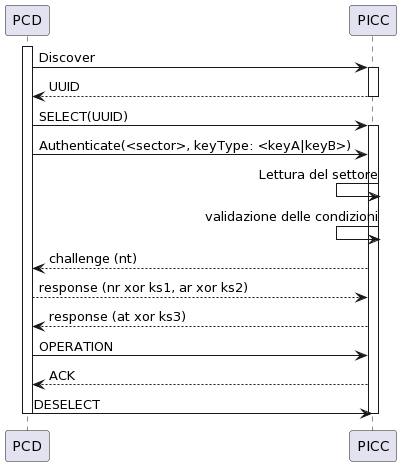
\includegraphics[width=40mm]{AuthSequence.png}
                    \caption{\scriptsize Diagramma di sequenza del processo di autenticazione a un blocco}
                    \label{fig:seq-three-pass-auth}
                \end{figure}
        \end{columns}
    }
\end{frame}
\note{
    Come è possibile vedere dallo schema, il processo di autenticazione inizia con il tag che invia un proprio nonce $n_t$ al lettore, in modo da - idealmente - impedire il riutilizzo di uno stato interno.
    Infatti il nonce è utilizzato in concomitanza con l'uid e la chiave del settore per inizializzare il cifrario.

    Infatti senza uuid e senza nonce, due tag con chiave uguale potrebbero essere scoperti solamente ascoltando (Eavesdropping) le comunicazioni.
    Inserend l'uuid nell'algoritmo ciò diviene impossibile perchè i tag avranno uno stato diverso in funzione dell'uuid che è unico (o comunque è improbabile che due tag abbiano lo stessu uuid)
    Ciò non ferma però eventuali attacchi che fanno leva sulla ripetizione degli stati iniziali del tag.

    A tal fine viene introdotto il numero casuale deciso dal tag: la sua trasmissione in chiaro non è direttamente un vettore di attacco, ma si vedrà che è stato il metodo utilizzato per scoprire svariate vulnerabilità sull'rng.
}

\begin{frame}[allowframebreaks]
    \frametitle{Three pass authentication sequence\cite{garcia2008dismantling}}
    In particolare la scelta dei nonce avviene come dalla seguente illustrazione, dove \(key\) è la chiave condivisa
    (ovvero la chiave che il lettore usa per autenticarsi)
    
    Generazione del tag nonce
    \[n_t = nextRandom()\]
    \[send(n_t)\]

    Dopo l'invio, sia il tag che il lettore inizializzano il proprio cifrario a flusso e computano i primi 32bit del \textit{keystream}
    \[ks_1 = cipherInit(key, uid, n_t)\]

    Generazione del reader nonce
    \[n_r = nextRandom()\]

    Invio del reader nonce (cifrato) e dalla risposta alla challeng così computata
    \[a_t = suc^2(n_t)\]
    \[ks_2 = cipher(n_r)\]
    \[send(n_r \oplus ks_1); send(a_t \oplus ks_2)\]
    
    Risposta finale
    \[send(suc^3(n_t) \oplus ks_3)\]

\end{frame}
\note{
    Sia la funzione \(suc(v)\) la successiva iterazione del rng con seed \(v\) 
    
    Il processo di scambio di chiavi viene così descritto:~\cite{nxpmifareev1datasheet}
    \begin{itemize}
        \item il tag sceglie il proprio nonce $n_t$ e lo invia al lettore
        \item entrambe le parti inizializzano il proprio cifrario con una funzione della chiave \(key\), \(n_t\) e l'uid del tag
        \item una volta ottenuto il nonce, il lettore computa i primi 32 bit del keystream, inserendo nel LFSR i 32 bit di una funzione $f(n_t, uuid)$
        \item il lettore genera \(n_r\) e lo invia al tag cifrandolo con \(ks_1\) (\(n_r \oplus ks_1\)) insieme invia la risposta alla challege \(a_r = suc^2(n_t)\) cifrata con i secondi 32 bit ottenuti aggiornando il proprio cifrario con $n_r$
        \item il tag quindi, aggiorna il proprio cifrario con \(n_r\) e verifica che $a_r$ sia valida.
        \item per completare l'autenticazione viene quindi inviato \(suc^3(n_t)\) cifrato con \(k_3\) in modo che Il lettore possa validare il tag.
    \end{itemize}
}



\section{Cifrari di flusso}
\begin{frame}
    ciao
\end{frame}


\section{CRYPTO1}

\subsection{Storia}

\begin{frame}
    \frametitle{Storia}
    \textbf{CRYPTO1} è uno stream cipher sviluppato da \textit{NXP~Semiconductors} nel 1994
    insieme alla famiglia di tag MIFARE Classic~\cite{tezcan2017brute}
\end{frame}


\begin{frame}
    \frametitle{Security through obscurity}
    La sicurezza del sistema era affidata al concetto di \textit{Security through obscurity}

    \begin{itemize}
        \item <2-> Metodo fortemente sconsigliato da tutti gli organi normativi sulla sicurezza\cite{scarfone2008guide}
        \item <3-> Tecnica in contrasto con \textit{Security by Design} e \textit{Open security}
    \end{itemize}
\end{frame}
\note{
    Contrariamente alle due politiche \textit{Security by Design} e \textit{Open security}
    la sicurezza tramite offuscamento è fortemente sconsigliata, in quanto affida la sicurezza del sistema
    al fatto che nessuno riesca a comprenderlo.

    Questa pratica rende quindi il sistema vulnerabile a qualsiasi attacco di tipo reverse engineering,
    oltre che a possibili fughe di informazioni.

    L'utilizzo di ideologie ``open'' permette la validazione del sistema da parte di un maggior numero di enti
    e di membri di una comunità, favorendo così l'individuazione di falle in minor tempo.

    Il metodo più efficiente, però, consiste sempre nell'utilizzo di sistemi già esistenti e ritenuti sicuri (p.e. tritium)
}

\begin{frame}
    \frametitle{La caduta di CRYPTO1}
    Nel 2008/2009 più ricercatori in contemporanea hanno trovato vulnerabilità e sono stati rilasciati attacchi sul critto-sistema CRYPTO1
    che ne hanno interamente distrutto la sicurezza.\cite{garcia2008dismantling}\cite{courtois2008algebraic}\cite{nohl2008reverse}\pause

    Il sistema presenta falle nella sicurezza in più settori:

    \begin{itemize}
        \item <2-> Random Number Generator
        \item <3-> Proprietà algebriche e vulnerabilità strutturali del LFSR
        \item <4-> Complessità delle chiavi (Che rendono il critto-sistema vulnerabile ad attacchi di tipo bruteforce~\cite{courtois2008algebraic})
        \item <5-> Logica di gestione della comunicazione
    \end{itemize}

    (Praticamente presenta falle in ogni sua componente)
\end{frame}


\subsection{Vulnerabilità}

\begin{frame}
    Le vulnerabilità trovate negli anni nel crittosistema sono le seguenti.

    Alcune di queste sono di facile soluzione perchè riguardano il lato hardware del lettore,
    per cui, a fronte di un costo maggiore, è possibile migliorarne le capacità.
\end{frame}

\begin{frame}
    \scriptsize
    \begin{itemize}
        \item <1-> Utilizzo di chiavi a 48 bit: Possibili attacchi BruteForce \cite{courtois2008algebraic}
        \item <2-> RNG del tag non è crittograficamente sicuro. infatti è un LFSR con condizione iniziale costante.
        \begin{itemize} \scriptsize
            \item <3-> Consegue che lo stato è prevedibile e dipende dal tempo trascorso dal poweron~\cite{garcia2008dismantling}\cite{courtois2008algebraic}
            \item <4-> Inoltre i numeri casuali sono generati a partire da 16 bit del registro 
            \item <5-> in particolare i numeri sono generati ad ogni ciclo di clock del tag, quindi la precisione del attaccante deve limitarsi a quanti di 10 microsecondi (106kHz) e la sequenza di numeri i ripete ogni 65535 iterazioni (0.6s)
        \end{itemize}
        \item <6-> L'RNG dei lettori viene aggiornato solamente ad ogni nuova autenticazione~\cite{garcia2008dismantling}
        \item <7-> La funzione di filtraggio del LFSR usa 20bit del registro e sono solo bit in posizione dispari
        \item <8-> LFSR State Recovery
        \item <9-> LFSR Rollback
        \item <10-> i bit di parità sono computati sul plaintext e poi inviati non cifrati
        \item <11-> nested authentication attacks
    \end{itemize}
\end{frame}


\subsubsection{LFSR}
\begin{frame}
    \frametitle{Dettagli sul LFSR}
    todo: 
        reverse engeneering \cite{nohl2008reverse} del chip per trovare il circuito di autenticazione
        attacchi per trovare la funzione \cite{garcia2008dismantling}
        attacchi dati dai odd
        nested auth e drschottky
\end{frame}

\subsubsection{Attacchi Algebrici}
\begin{frame}
    \frametitle{Attacchi Algebrici}

\end{frame}


\subsection{Attacchi}
\subsubsection{Genuine Reader}
\begin{frame}
    \frametitle{LFSR Recovery (Genuine Reader Attack)}
    Data la dimensione ridotta del LFSR è possibile creare una tabella contenente le coppie ($LFSR_{value}$, $KeyStream$) per tutti gli stati da \texttt{0x000000000000} a \texttt{0x000FFFFFFFFF} ($2^{36}$ righe)\pause

    Successivamente si effettua un tentativo di autenticazione simulando un tag, inviando all'inizio dela trasmissione un nonce $n_t$ nella forma \texttt{0x0000XXX0} (4096 tentativi) senza procedere oltre al primo passaggio\pause
    
    Questo causa l'invio di un comando di halt da parte del lettore (comando noto) cifrato con lo stato attuale dal quale possiamo ricavare $ks_3$ e $ks_2$ dalla risposta $suc^2(n_t)$
\end{frame}
\note{
    Come è possibile osservare dalla figura \ref{fig:crypto1} la funzione f non dipende dai valori terminali del LFSR.
    
}
\begin{frame}
    \frametitle{LFSR Recovery (Genuine Reader Attack)}
    Data la struttura è stato notato come esista un valore di $n_t$ tale per cui lo stato del LFSR equivale a \[\texttt{0xYYYYYYYY000Y}\]\pause

    Il lettore quindi aggiorna il cifrario con il valore di $n_r$, che causa gli zeri nel LFSR di raggiungere lo stato \[\texttt{0x000YZZZZZZZZ}\]\pause

    Possiamo quindi trovare lo stato del LFSR dalla tabella cercando per i valori di $ks_2$ e $ks_3$
\end{frame}

\begin{frame}
    \frametitle{LFSR Rollback (Genuine Reader Attack)}
    Dato un qualsivoglia stato del LFSR è possibile ottenere lo stato dell'iterazione precedente conoscendo quanto è stato inserio.
    \pause

    Una volta ottenuto lo stato del LFSR dopo l'inserzione del nonce $n_r$ non è ancora possibile effettuare il rollback perchè $n_r$ è cifrato.
    \pause
    
    La vulnerabilità viene utilizzata ora: Dato che l'MSB del LFSR non è input della funzione di filtro $f$ (Vedi figura~\ref{fig:crypto1})
    è possibile sostituirlo con un valore $r$ senza effetti collaterali.
    \pause
    
    Ciò permette di ottenere il $n_{r31}$.
    Utilizzando questo valore è quindi possibile ricalcolare il valore di $r$
\end{frame}
\note{
    vedi \cite{garcia2008dismantling},
    la relazione è \[rk+48 = rk \oplus rk+5 \oplus rk+9 \oplus rk+10 \oplus rk+12 \oplus rk+14 \oplus rk+15 \oplus \]\[rk+17 \oplus rk+19 \oplus rk+24 \oplus rk+27 \oplus rk+29 \oplus rk+35 \oplus rk+39 \oplus rk+41 \oplus rk+42 \oplus rk+43 \oplus i.\]
}

\subsubsection{Genuine Tag}
\begin{frame}
    \frametitle{Genuine Tag Attack}
    Sfruttando la vulnerabità relativa al leak di informazioni all'invio di un NACK~\ref{sec:parity-bit-vuln} è possibile utilizzarla al fine di ottenere 
    la chiave utilizzata dal tag.\pause

    Ottenendo il NACK cifrato è possibile ottenere 4 bit di keystream.\pause

    \textit{Fissando un nonce $n_t$ e un prefisso di 24 bit sulla risposta alla challenge $a_t$ che ha dato un NACK, esiste una probabilità di 1/12.8 che il keystream non dipenda dal quarto byte decifrato.}\cite{Courtois2009TheDS}
\end{frame}

\begin{frame}
    \frametitle{Genuine Tag Attack}
    A questo punto è possibile sfruttare il fatto che l'RNG sia predicibile in funzione del Power On Time:
    Mantenendo $n_t$ costante insieme ai primi 24 bit della risposta ritentiamo l'autenticazione per 256 volte 
    (variando quindi il quarto byte della risposta) ottenendo così circa 8 risposte da parte del tag.\pause

    A queso punto è dimostrabile che, assumendo che il keystream non dipenda dalla decifratura del quarto byte (P = 1/12.8), allora
    la differenza degli stati dipende da una funzione della differenza di c3\cite{Courtois2009TheDS}\pause

    Con queste risposte è possibile clcolare la differenza dello stato per tutti i tentativi
\end{frame}

\begin{frame}
    \frametitle{Genuine Tag Attack}
    A questo punto è necessario individuare i 21 bit dello stato che determineranno i bit a seguire, dove per ogni risposta del tag
    potremo dividere la dimensione dello spazio di ricerca di 4.\pause

    Seppur un attacco complesso e basato su proprietà sttistiche, è possibile ottenere la chiave di autenticazione a un settore in circa 4000 query (30 minuti)\pause

    È possibile trovare una implementazione qui: \href{https://github.com/DrSchottky/mfcuk/blob/master/src/mfcuk.c\#L623}{https://github.com/DrSchottky/mfcuk/}
\end{frame}

\subsubsection{Nested Authentication}
\begin{frame}
    \frametitle{Nested authentication}\label{sec:nested-auth}
    Autenticazioni successive seguono lo stesso protocollo ma $n_t$ viene inviato cifrato con il nuovo stato derivato dalla chiave di autenticazione
    caricata nel LFSR\pause

    Un possibile attacco potrebbe essere il bruteforcing dei 65536 possibili valori casuali\pause

    Utilizzando la vulnerabilità dove i bit di parità sono cifrati con un bit condiviso del keystream (Slide~\ref{sec:parity-enc}) possiamo dedurre che
    \[n_t = {b_{31},b_{30}, ... b_1, b_0}\]
    \begin{multline*}
        transmission_stream = \{b_0, b_1 ... b_7, p_0, b_8 ... b_{15}, p_1, \\ b_{16} ... b_{23}, p_2, b_{24} ... b_{31}, p_3\}
    \end{multline*}

\end{frame}

\begin{frame}
    \frametitle{Nested authentication}
    Dalla precedente vale
    \begin{math}
        \begin{cases}
            p_0 = rp_0 \oplus ks_8\\
            b_8 = rb_8 \oplus ks_8\\
            p_1 = rp_1 \oplus ks_{16}\\
            b_{16} = rb_{16} \oplus ks_{16}\\
            p_2 = rp_2 \oplus ks_{24}\\
            b_{24} = rb_{24} \oplus ks_{24}\\
        \end{cases}
    \end{math}
\end{frame}

\begin{frame}
    \frametitle{Nested authentication}
    Dalla quale possiamo dedurre
    \begin{math}
        \begin{cases}
            p_0 \oplus b_8 = rb_8 \oplus rp_0\\
            p_1 \oplus b_{16} = rb_{16} \oplus rp_1\\
            p_2 \oplus b_{24} = rb_{24} \oplus rp_2\\
        \end{cases}
    \end{math}\pause

    Di conseguenza è possibile ricavare se il bit di parità del byte precedente è uguale al primo bit del secondo byte, dimezzando lo spazio di ricerca
    per ogni bit di parità (per un totale di una riduzione di un fattore pari a 8)\pause

    Nel caso di una comunicazione tra lettore e tag genuini è possibile ridurre lo spazio di ricerca ulteriormente grazie alla successiva risposta del tag contenente 7 bit di parità,
    portando così i nonce candidati a 64.
\end{frame}
\note{
    addizionalmente è possibile prevedere il valore del nonce data la bassa entropia del rng e la sua predicibilità
}
\subsection{Considerazioni}
\begin{frame}
    \frametitle{Considerazioni}
    MIFARE Classic non rappresenta una piattaforma sicura per lo sviluppo di applicazioni contactless, e in
    particolare è inadatto ad applicazioni relative a micropagamenti\pause

    Durante la progettazione della tecnologia sono stati commessi gravi errori che, data la banalità di alcuni,
    potrebbero essere stati inseriti con scopi malevoli~\cite{Courtois2009TheDS}
\end{frame}

\subsubsection{RNG}
\begin{frame}
    \frametitle{Miglioramenti - RNG}
    La maggioranza degli attacchi utilizza la predicibilità del RNG. \pause
    
    La soluzione in questo caso è di utilizzare un TRNG disponibile in hardware, a costo di spazio su silicio e di costi pecuniari maggiorati.\pause

    Un miglioramento parziale potrebbe avvenire utilizzando un LFSR da 32 bit e non 16, aumentando così le possibili combinazioni al fine di rallentare gli attacchi.
\end{frame}

\subsubsection{TRNG}
\begin{frame}[allowframebreaks]
    \frametitle{TRNG}
    \begin{figure}
        \centering
        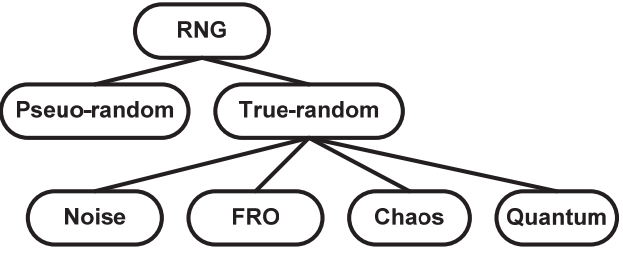
\includegraphics[width=.3\textwidth]{rngFamilies.png}
        \caption{Famiglie di RNG}
    \end{figure}
    È possibile creare TRNG basati sul rumore dell'ambiente in relativamente poco spazio e a basso costo.~\cite{fermevc2016low}

    Il concetto principale nella generazione consiste nel generare un rumore bianco casuale dall'ambiente circostante o da una giunzione PN.

    Ciò permette di generare valori metastabili all'ingresso di flipflop 
    che potranno generare risultati non deterministici per gli effetti elettronici interni.

    \begin{figure}
        \centering
        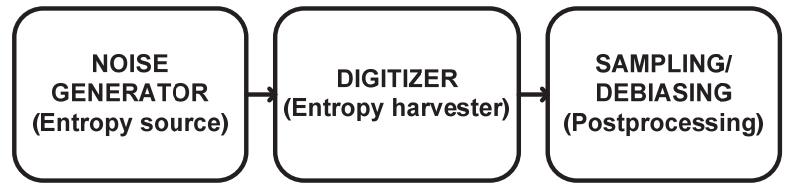
\includegraphics[width=.5\textwidth]{trng_noise.png}
        \caption{Processo di generazione di un numero casuale.}
    \end{figure}

    Da quanto riportato da~\cite{fermevc2016low} è possibile implementare un TRNG con componenti comuni e a bassissimo costo (LM393) e un microcontrollore (già presente nel tag).

    \begin{figure}
        \centering
        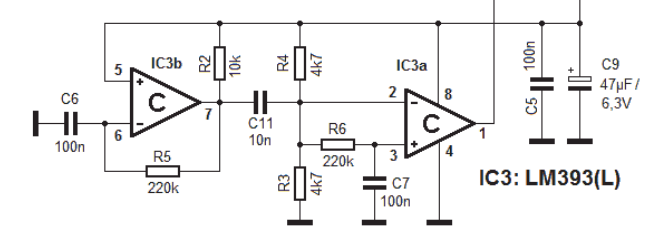
\includegraphics[width=.5\textwidth]{trng_schematic.png}
        \caption{Schema elettronico del generatore di rumore.\cite{fermevc2016low}}
    \end{figure}

    Senza andare nel dettaglio del funzionamento, il primo comparatore viene utilizzato come vera e propria fonte di entropia, mentre il secondo viene utilizzato come digitalizzatore per avere un output binario.

    \begin{figure}
        \centering
        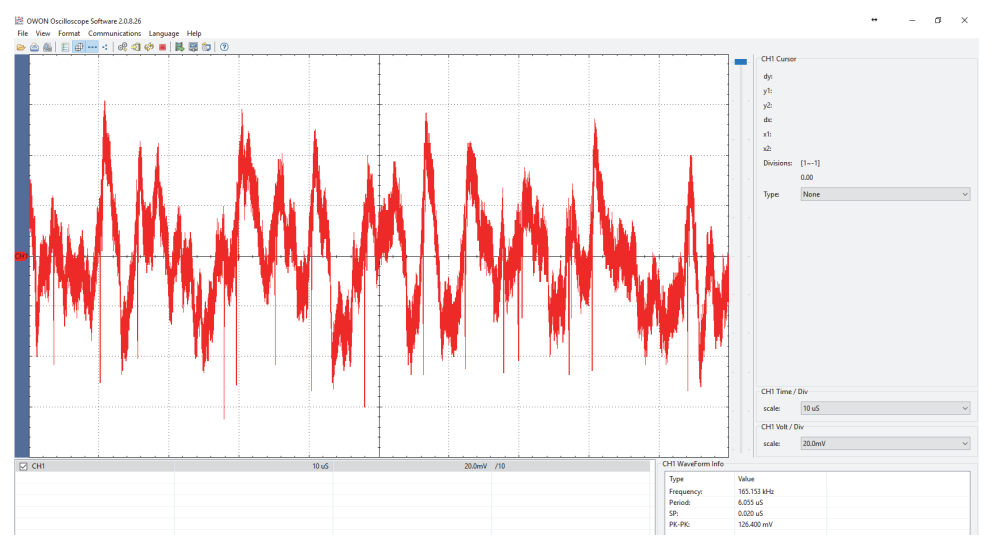
\includegraphics[width=.4\textwidth]{trng_noise_oscope.png}
        \caption{Traccia del rumore generato.\cite{fermevc2016low}}
    \end{figure}

    Svantaggi: Il consumo di un generico TRNG si aggira sui 100mW~\cite{fermevc2016low}. Sono necessarie modifiche e ottimizzazioni per l'inclusione in un tag passivo.
\end{frame}

\subsubsection{LFSR}
\begin{frame}
    \frametitle{Miglioramenti - LFSR}
    Alcune vulnerabilità sono causate dalla funzione di filtraggio del LFSR (Slide~\ref{sec:filter-fn}).
    A tal fine potrebbe essere vantaggiosa un'implementazione dove il cifrario venga sostituito da un modello crittograficamente sicuro.
    
    Una valida proposta potrebbe essere GRAIN-128, cifrario ideato sostanzialmente per ambienti e dispositivi a basso costo e bassissima area occupata\cite{gren2011grain}\cite{sonnerup2019efficient}
\end{frame}

\begin{frame}
    \frametitle{Miglioramenti - LFSR}
    Restano però alcune problematiche:
    \begin{itemize}
        \item <1-> Grain necessita di una chiave di 128bit\newline
                A tal fine è possibile caricare un valore randomico a seguire della chiave nel cifrario per garantire più entropia dei processi di autenticazione.
        \item <2-> Alternativamente sarebbe necessario aumentare la lunghezza della chiave.\newline Per fare ciò sarebbe poi necessario modificare la struttura di memoria oppure ridurre lo spazio consentito ai dati del tag.
    \end{itemize}
\end{frame}
\note{
    In ogni caso la lunghezza della chiave di 48 bit è da considerarsi non siura, tanto quanto la tecnologi hardware.
}

\subsubsection{Grain128}
\begin{frame}[allowframebreaks]
    \frametitle{Grain128a}
    \textbf{Vantaggi}
    \begin{itemize}
        \item <1-> Crittograficamente sicuro
        \item <2-> Può includere un MAC
    \end{itemize}

    Grain utilizza chiavi da 128 bit e IV da 96 bit, mentre la struttura interna è composta da un LFSR da 128 bit e da un NLFSR anch'esso da 128 bit

    \begin{figure}
        \centering
        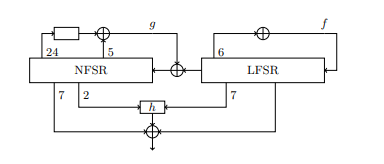
\includegraphics[width=.5\textwidth]{grain128.png}
        \caption{Schema logico di Grain128/Grain128a}
    \end{figure}

    All'interno di Grain è possibile trovare due registri a scorrimento, uno lineare e uno non lineare.

    In aggiunta $h$ è una funzione non lineare che contribuisce all'output.
\end{frame}

\begin{frame}
    \frametitle{Grain128a iii}

    Per inizializzare il cifrario, una chiave da 128bit e un IV da 96 bit vengono inseriti nell'NLFSR e nel LFSR rispettivamente, completando l'LFSR con una costante.
\end{frame}

\begin{frame}
    \frametitle{Grain128a - Autenticazione i}

    Per autenticare il tag è possibile utilizzare il cifrario Grain128a:

    Il keystream è dato da $y_{64+2n}$ ovvero dai bit dispari dell'output scartando i primi 64.

    \begin{figure}
        \centering
        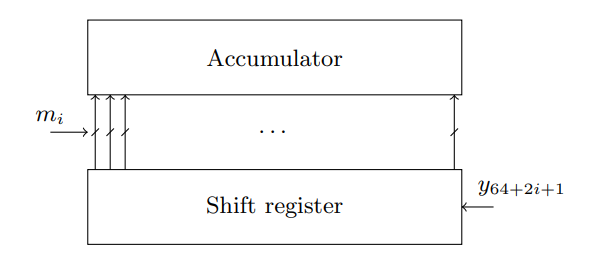
\includegraphics[width=.5\textwidth]{grain128auth.png}
        \caption{Schema logico dell'autenticazione utilizzata da Grain128a}
    \end{figure}
\end{frame}

\begin{frame}
    \frametitle{Grain128a - Autenticazione ii}

    Assumiamo di avere un messaggio $\bar{m} = m_0,m_1,...,m_{L-1}$ di lunghezza $L$.

    Per garantire che $\bar{m}$ e $\bar{m}||0$ abbiano risultato diverso (attacchi di tipo extension) poniamo $m_L = 1$\pause

    \textbf{Inizializzazione}

    Il registro accumulatore viene inizializzato con i primi 32 bit del keystream, il registro a scorrimento viene inizializzato con i successivi 32.\pause

    \textbf{Autenticazione}

    Codificando il messaggio, il registro a scorrimento sarà aggiornato ogni due bit del keystream ($r_{i+31 = y_{64+2i+1}}$) mentre l'accumulatore sarà aggiornato secondo $a_{i+1} = a_i \oplus m \cdot r$
\end{frame}
\note{
    Il risultato dell'autenticazione è quindi il valore finale dell'accumulatore che sarà uguale sia per la cifratura che la decifratura del messaggio.
}

\begin{frame}
    \frametitle{Miglioramenti - ALGORITMO}
    Una soluzione più drastica è rappresentata dal cambio del circuito di cifratura, passando a un'implementazione AES a basso costo.\cite{feldhofer2005aes}

    In questo caso resta la problematica della gestione di chiavi a 128 bit.
\end{frame}


\subsection{Successori}
\begin{frame}
    \frametitle{Successori}
    \begin{itemize}
        \item <1-> MIFARE Plus: Drop-in replacement con algoritmo modificato AES-128. Data la compatibilità con sistemi MIFARE Classic senza supporto ad AES, presenta ancora tutte le vulnerabilità precedentemente discusse
        \item <2-> MIFARE DesFire: Utilizza AES e DES/3DES per garantire la sicurezza ma notevolmente più costose: utilizzano un microcontrollore sul quale è possibile eseguire un sistema operativo. Permettono quindi di essere usate come SecureElements
    \end{itemize}
\end{frame}



\section{Bibliografia}
\begin{frame}[allowframebreaks]
    \frametitle{Bibliografia}
    \bibliography{texmf/bibtex/bib/refs}
\end{frame}
\end{document}
